\documentclass[10pt]{article}
\usepackage{caption}
\usepackage{amsmath}
\usepackage{array}
\usepackage{url} 
\usepackage{enumerate}
\usepackage[linesnumbered,ruled,vlined]{algorithm2e}
\usepackage{longtable}
\usepackage{multirow} % tables
\usepackage{rotating} % for rotating texts
\usepackage{subfigure}
\usepackage{float}
\usepackage{paralist}
\usepackage{amsfonts}
\pagestyle{empty} % hiding page numbering
\sloppy % for tricky allignments
\usepackage[justification=centering]{caption}
\usepackage{longtable}

\newcolumntype{L}[1]{>{\raggedright\let\newline\\\arraybackslash\hspace{0pt}}m{#1}}
\newcolumntype{C}[1]{>{\centering\let\newline\\\arraybackslash\hspace{0pt}}m{#1}}
\newcolumntype{R}[1]{>{\raggedleft\let\newline\\\arraybackslash\hspace{0pt}}m{#1}}

\DeclareMathOperator*{\argmax}{arg\,max}

\usepackage[a4paper, margin=0.75in]{geometry}
 
\newcommand{\doctitle}{Study of Three State-of-the-art Image Colorization Techniques of Last Three Decades}


\title{\textbf{\doctitle}\\ \vspace{3mm}
Term Paper: CSci 5561 - Computer Vision}
\author{Md Jahidul Islam (5188102)}

\date{}
\begin{document}
\maketitle

\begin{abstract}
Our project (team: YAL) is on designing a generative adversarial network (GAN) based model for automatic image colorization. I worked on the generator part; while doing so, I explored three colorization algorithms, which have been considered the state-of-the-art over three different time-spans. This report briefly discusses these algorithms, related implementation issues, results, and lessons learned while exploring these methods.    
\end{abstract}

\section{Introduction}\label{sec:intro}
Image colorization \cite{zhang2016colorful, cheng2015deep, bugeau2014variational} refers to colorizing a given gray-scale image so that it appears real. 
A large amount of photographs, videos and movies, mainly antique, lack color; image colorization can provide a modern and vivid view to these images. In addition, surveillance cameras often capture (or store) gray-scale images for convenience. Several underwater inspection and surveillance applications \cite{lu2013underwater, torres2005color} often have to deal with color-less images due to lack of visible light in deep-water. Robust and efficient image colorization techniques can be used in these applications with substantial benefits.   

\begin{figure}[h]
\centering
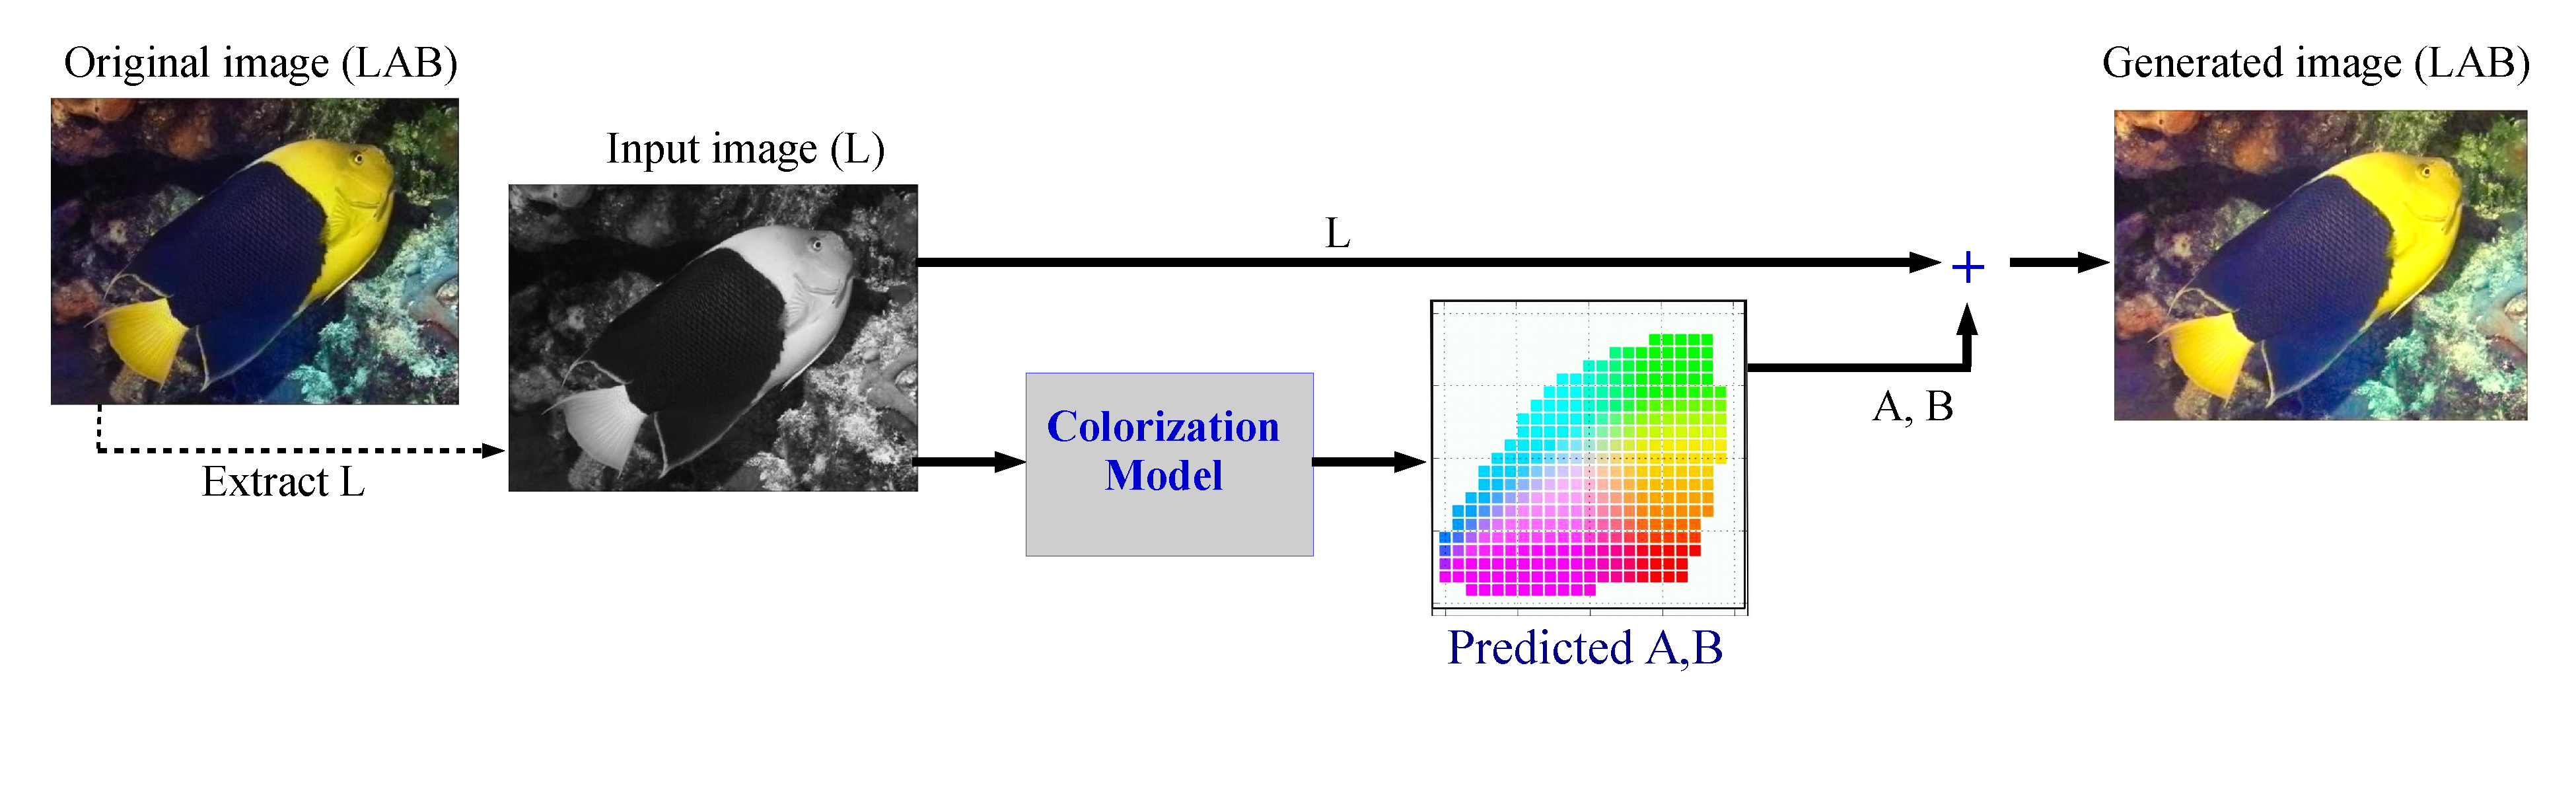
\includegraphics[width=\linewidth]{Figs/6.pdf}
\vspace{-13mm}
\caption{Basic image colorization procedure is shown. LAB color-space is generally used for convenience (\textit{i.e.}, one less unknown dimension); given the lightness channel $L$, task for the colorization model is to predict $A$ and $B$ channels so that the colorized image appears natural. (Further discussion on discretized values for $A$, $B$ channels are provided in Section \ref{sec:res}) }
\label{fig:col}
\end{figure}  

Colorizing a gray-scale image (\textit{i.e.}, only intensity values are known) is a difficult and ill-posed problem. Computer vision community have approached this problem in different ways over the last few decades \cite{zhang2016colorful, cheng2015deep, bugeau2014variational, charpiat2008automatic, luan2007natural, konushin2006interactive}. Before the advent of deep-learning \cite{lecun2015deep}, researchers have tried many classical techniques \cite{charpiat2008automatic, luan2007natural, konushin2006interactive, levin2004colorization, lagodzinski2008digital} to capture relationships between color components ($RGB$ or $LAB$) and image level features. 
Due to multi-modality and ill-posed nature of the problem, optimization based techniques \cite{levin2004colorization, charpiat2008automatic} and probabilistic models \cite{lagodzinski2008digital} were the only ones that achieved decent colorization performance in few specific applications. 
However, overall performance of these techniques, in general, were still poor due to the high non-linearity and abstract nature of color-feature relationship.  

Recently, deep-learning based image colorization techniques \cite{zhang2016colorful, cheng2015deep, varga2016fully, li2017watergan}, trained over millions of images, have shown significantly better performance over the earlier classical methods. For instance, the current state-of-the-art, `colorful colorization' \cite{zhang2016colorful}, can fool a human observer $32\%$ of the time in a \textit{colorization Turing-test} scenario. Additionally, the generalized performance of these techniques in different lighting conditions is also very good. 

However, there are still plenty of rooms for improvement. In our project, we explored GAN-based models for colorization. GAN \cite{goodfellow2014generative} is a generator-discriminator  framework for adversarial learning. Many learning-based applications have experienced a significant boost in performance with such adversarial learning. While details of our project will be discussed in the project report, this report discusses three papers I explored while working with the generator of our model.  

The rest of the report is organised as follows: first, the background and related work is presented in Section \ref{sec:back}. Subsequently, a detailed discussion on the three relevant colorization algorithms is presented in Section \ref{sec:approaches}. Finally, the adopted scheme, implementation details, and related results are presented in Section \ref{sec:res}. 

\section{Background and Related Work}\label{sec:back}
As mentioned in the previous Section, image colorization is an ill-posed problem due to multi-modality and ambiguity. 
While some natural objects commonly hold the same color (e.g grass is \textit{usually} green), many are left up for interpretation. 
For example, given a gray-scale image of someone wearing a dark colored shirt, 
there is no way of figuring out the true color. 
Instead, the objective is to come up with a colorization that appears real, \textit{i.e.}, natural. 

User-based approaches \cite{levin2004colorization, konushin2006interactive, reinhard2001color, vrhel1992color} were popular for being fast and relatively accurate as user can provide a good prior for the inherent color distribution. However, these methods are not applicable for large scale automatic colorization, which led researchers to adopt optimization and probabilistic approaches \cite{charpiat2008automatic, bugeau2014variational, lagodzinski2008digital}. 
These approaches model a likelihood based color approximation for each pixel given the neighborhood information. 
Few methods introduce additional step for spatial coherency through image based segmentation as well. However, overall colorization performance of these approaches are not very appealing \cite{deshpande2015learning} for general usage in a large scale. This is because the prior distribution of color-space is domain-dependant; for instance, face images, underwater images, outdoor and satellite images, all have different color distributions. Besides, it is difficult to capture the highly non-linear and abstract color-feature relationships without large-scale training. 

\begin{figure}[h]
\centering
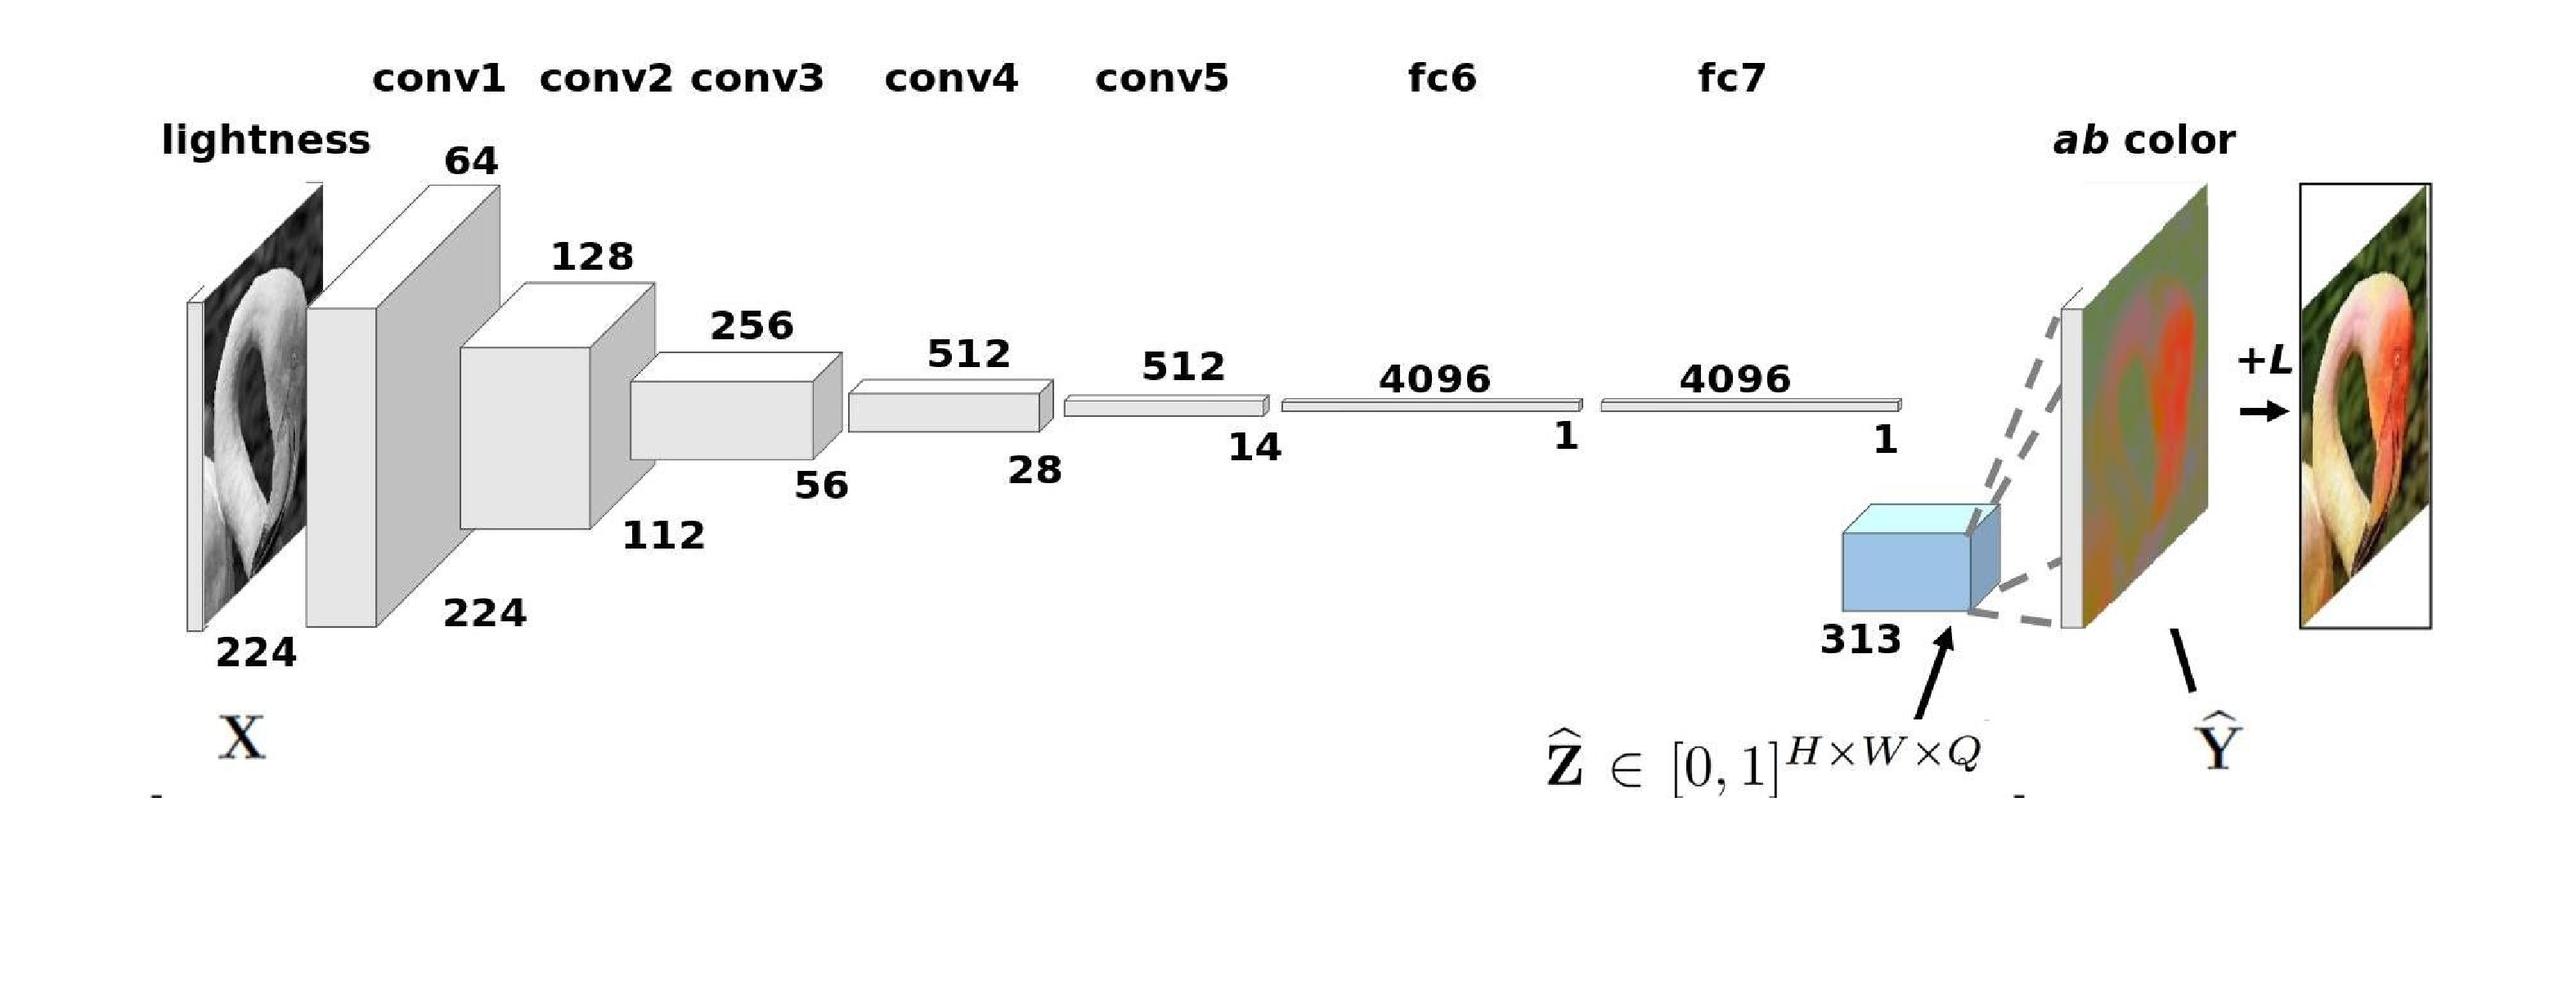
\includegraphics[width=\linewidth]{Figs/7.pdf}
\vspace{-16mm}
\caption{A simple architecture \cite{zhang2016colorful} for image colorization with $5$ convolutional and $2$ fully connected layers. Given input $X$ (gray-scale image $224$ $\times$ $224$), the first layer generates $64$ feature maps, second layer $128$ feature maps, and so on. Spatial down-sampling is performed through layers to capture more abstract features; eventually, up-sampling to appropriate dimensions is performed at the final layer to predict $A$, $B$ values  ($Z$) for each pixel. }
\label{fig:col}
\end{figure} 



In recent times, deep-learning based approaches \cite{zhang2016colorful, cheng2015deep, varga2016fully, li2017watergan} have produced significantly better colorization performance as they can extract highly non-linear spatial relationships if trained over large datasets. 
The convolutional layers learn appropriate filters 
to produce good feature-space representations from raw images. 
These feature extraction and filtering is performed over multiple layers 
to explore complex spatial relationships within the image-space. 
Often fully connected layers are used for classification or object recognition tasks. 
However, for image-to-image translation tasks such as colorization, it is common to use only convolutional layers \cite{zhang2016colorful, cheng2015deep}. Figure \ref{fig:col} shows a simple architecture for image colorization and overall transition of feature maps over layers. Detailed discussion on how the training is done and colorization is achieved, is provided in Section \ref{sec:res}. 


\section{Relevant Aproaches and Implementation Issues}\label{sec:approaches}
As mentioned in the previous Section, state-of-the-art image colorization techniques were based on  probabilistic and optimization models during the last two decades (1995-2015). Current state-of-the-art is based on deep-learning, which exhibits significant boost in performance. These algorithms provide a chronological insight of how colorization techniques in the literature have evolved over the years. 
This report focuses on the following three algorithms: 
\textit{colorization using optimization} \cite{levin2004colorization}, \textit{colorization via multimodal predictions} \cite{charpiat2008automatic}, and \textit{colorful image colorization} \cite{zhang2016colorful}. 


\subsection{Colorization using Optimization (2004)}
Colorization using optimization \cite{levin2004colorization} is one of the first algorithms that achieved good colorization performance. It is based on the assumption that similar regions (i.e, intensity values) in the image-space are likely to have similar colors. An optimization problem based on \textit{quadratic cost function} is formed to govern image segmentation and tracking of similar regions. 
The target is to minimize the difference between 
color $U(r)$ at pixel $r$ and weighted average of
colors at neighboring pixels, using the cost function: $ C(U) = \sum_r [ U(r) - \sum_{s \in Nighbor(r)} U(s) \cdot w_{rs}  ]^2 $.  (here, $w_{rs}$ is a Gaussian kernel)

\vspace{1mm}
This method is fast and performance is decent enough; however, it is not automatic. That is, user provides a patch of colors within the image-space to begin with- which significantly boosts the performance. First, the user indicates a template by scribbling the desired color in the interior of the region. Then, using these user supplied markers, this technique automatically propagates colors to the remaining pixels in the image sequence. A demonstration is illustrated in Figure \ref{fig:res1}.


\begin{figure}[h]
\centering
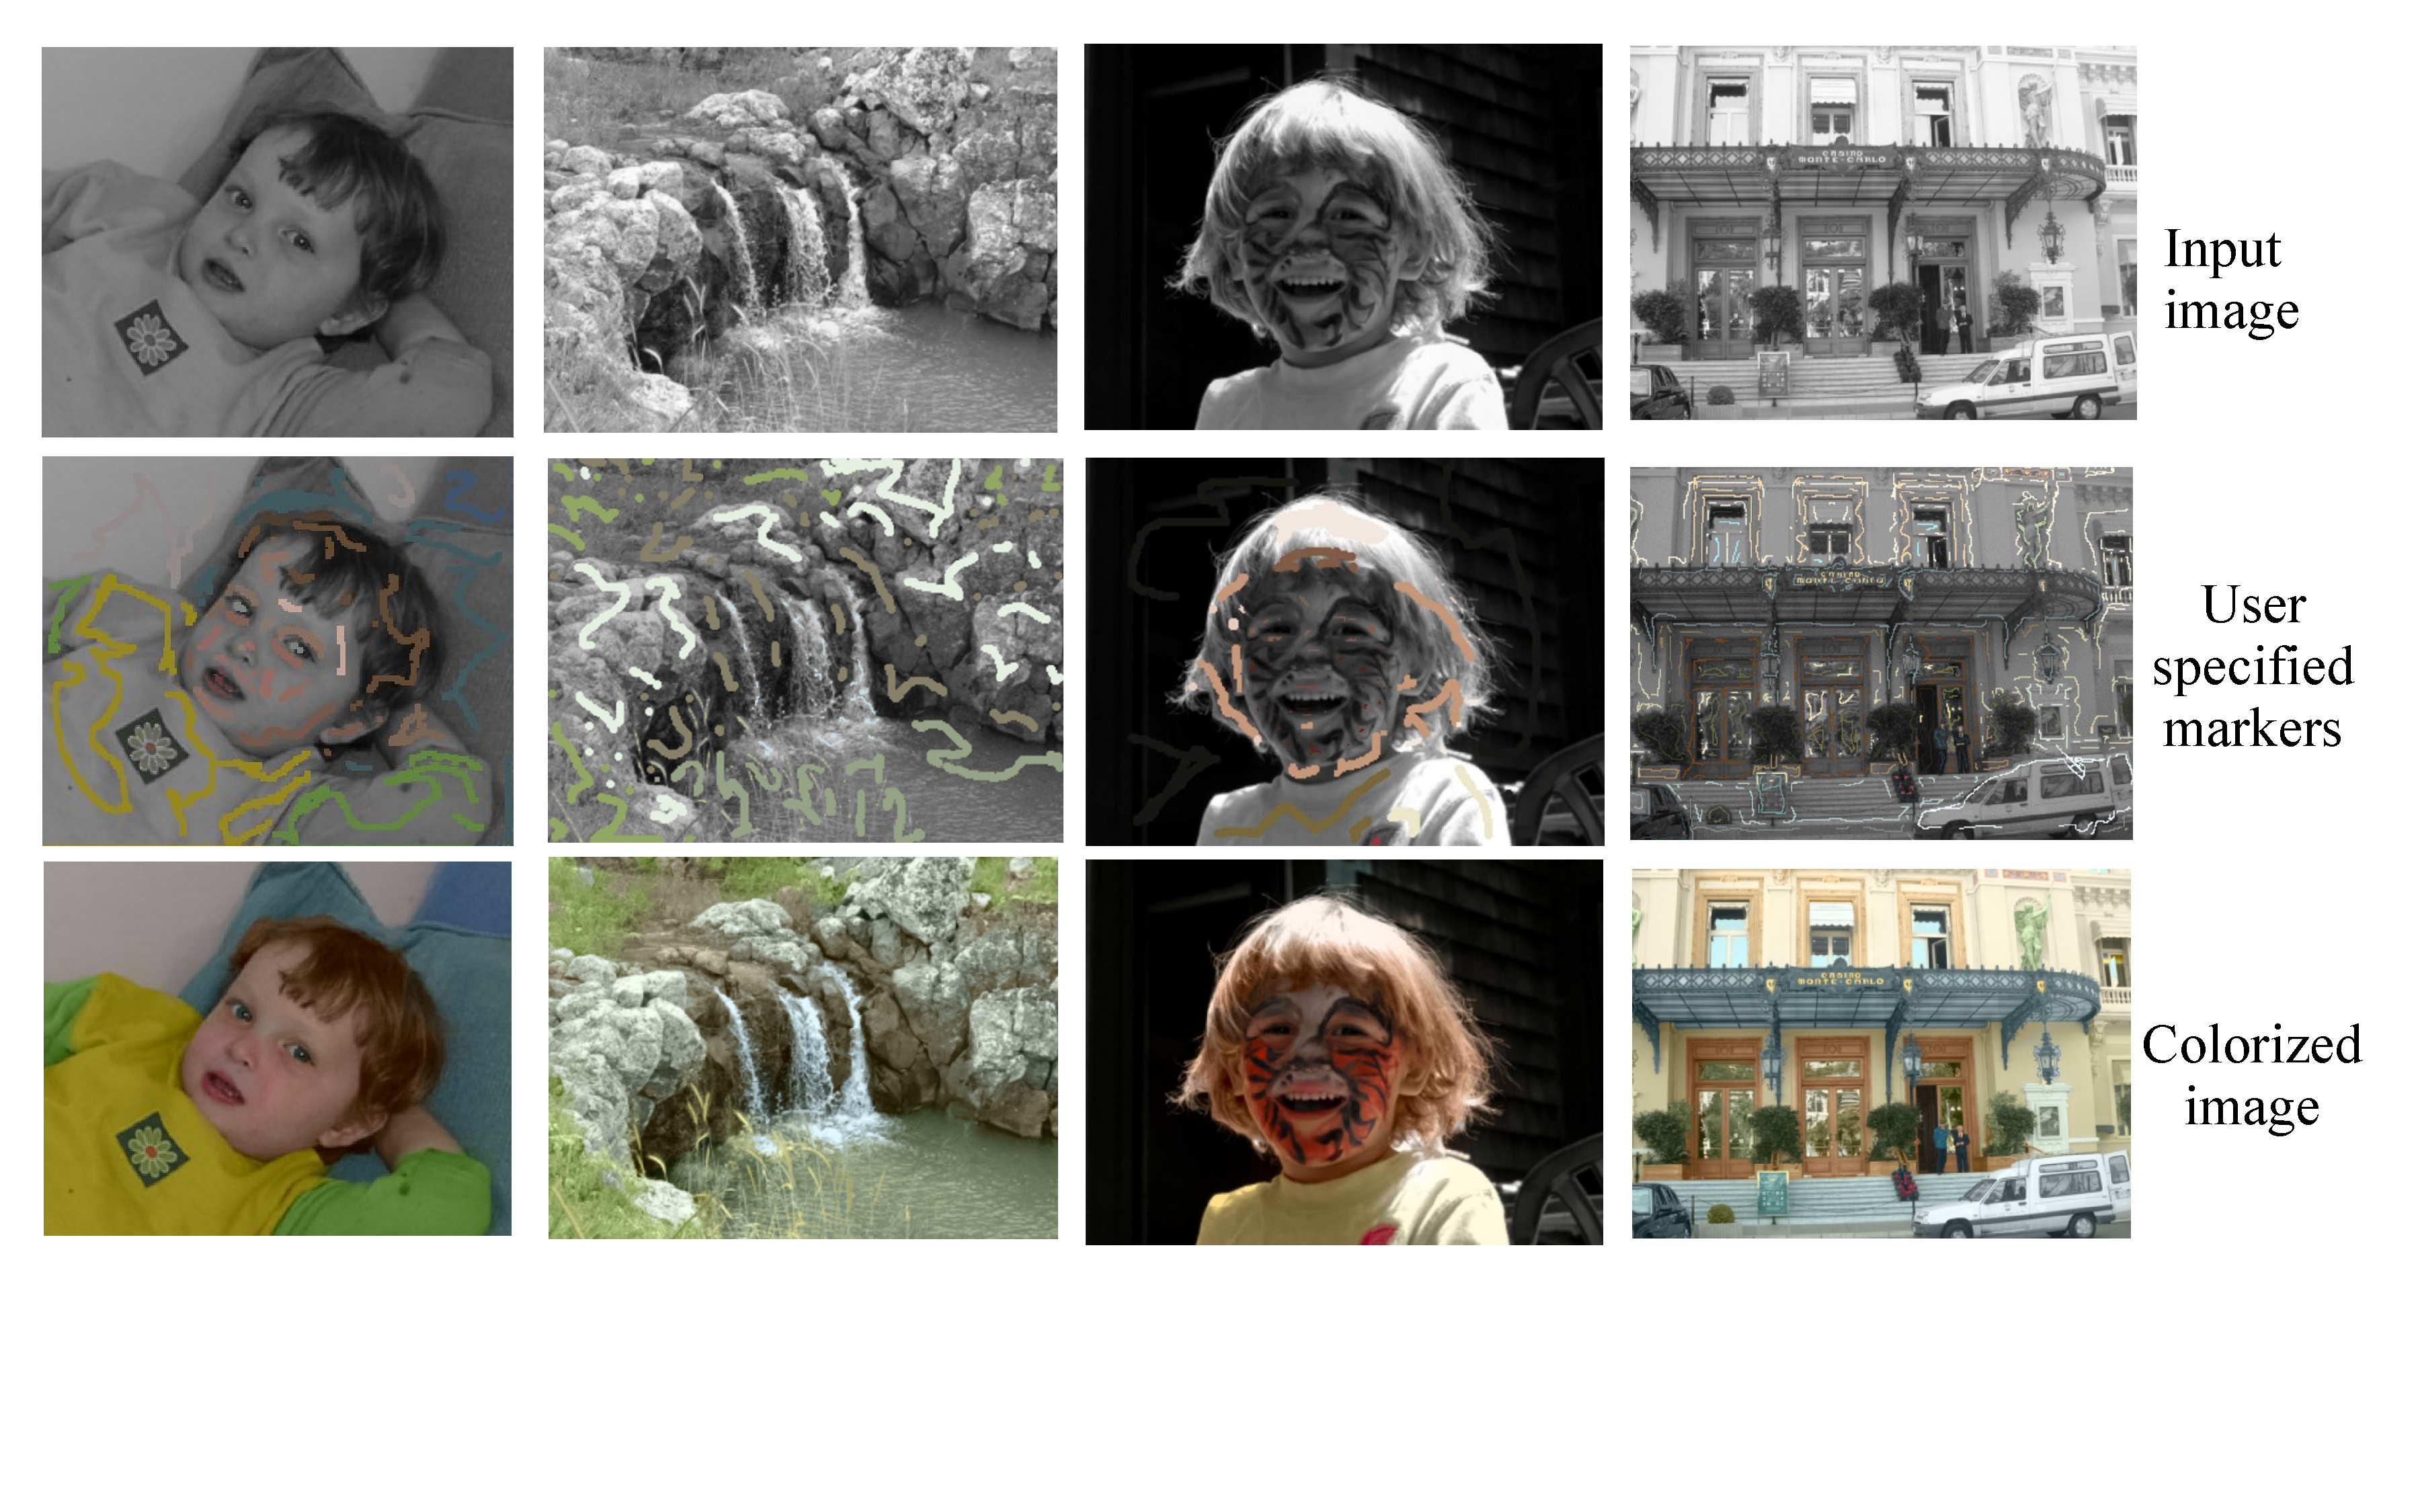
\includegraphics[width=\linewidth]{Figs/5.pdf}
\vspace{-20mm}
\caption{Demonstrations of how colorization is performed in \cite{levin2004colorization} using user-specified markers (code is available at \cite{AnatCol}) }
\label{fig:res1}
\end{figure} 


\subsubsection{Pros and Cons:}
This technique introduces a clever way for assigning colors to similar regions in the image-space, without explicitly performing computationally expensive image based segmentation. Additionally, it is fast and colorization is spatially coherent.  
However, such insuitions are not readily applicable or extendible automatic image colorization techniques (such as ours). Therefore, it is not suitable for large scale image colorization. 

\subsection{Automatic Image Colorization via Multimodal Predictions (2008)}
Automatic image colorization via multimodal predictions \cite{charpiat2008automatic} works as follows: first, it discretizes the color-space ($LAB$) into $73$ bins and measures approximate distribution of colors for each pixel based on the training data. 
Then, each local description around a pixel is modeled by a $30$-dimensional vector based on SURF descriptor. 
Subsequently, both the distribution of color-space and corresponding feature vectors are fed to a color predictor. 
The conditional probability of the color $c_i$ at pixel $p$, given the local description
$\textbf{v}$ of its grey-scale neighborhood is expressed as: $P(c_i|\textbf{v}) = [\sum_{j:c_j \in B_i}{K(\textbf{v}_j, \textbf{v})} /  \sum_j {K(\textbf{v}_j, \textbf{v})} ]$, where $B_i$ denotes the color bins and $K$ is a Gaussian kernel.

Following the prediction, a refinement step is performed 
based on expected variation of color at each pixel. 
Finally, graph-cut algorithm is used to refine the image coloring at the global level. 
A demonstration is illustrated in Figure \ref{fig:res1}.

\begin{figure}[h]
\centering
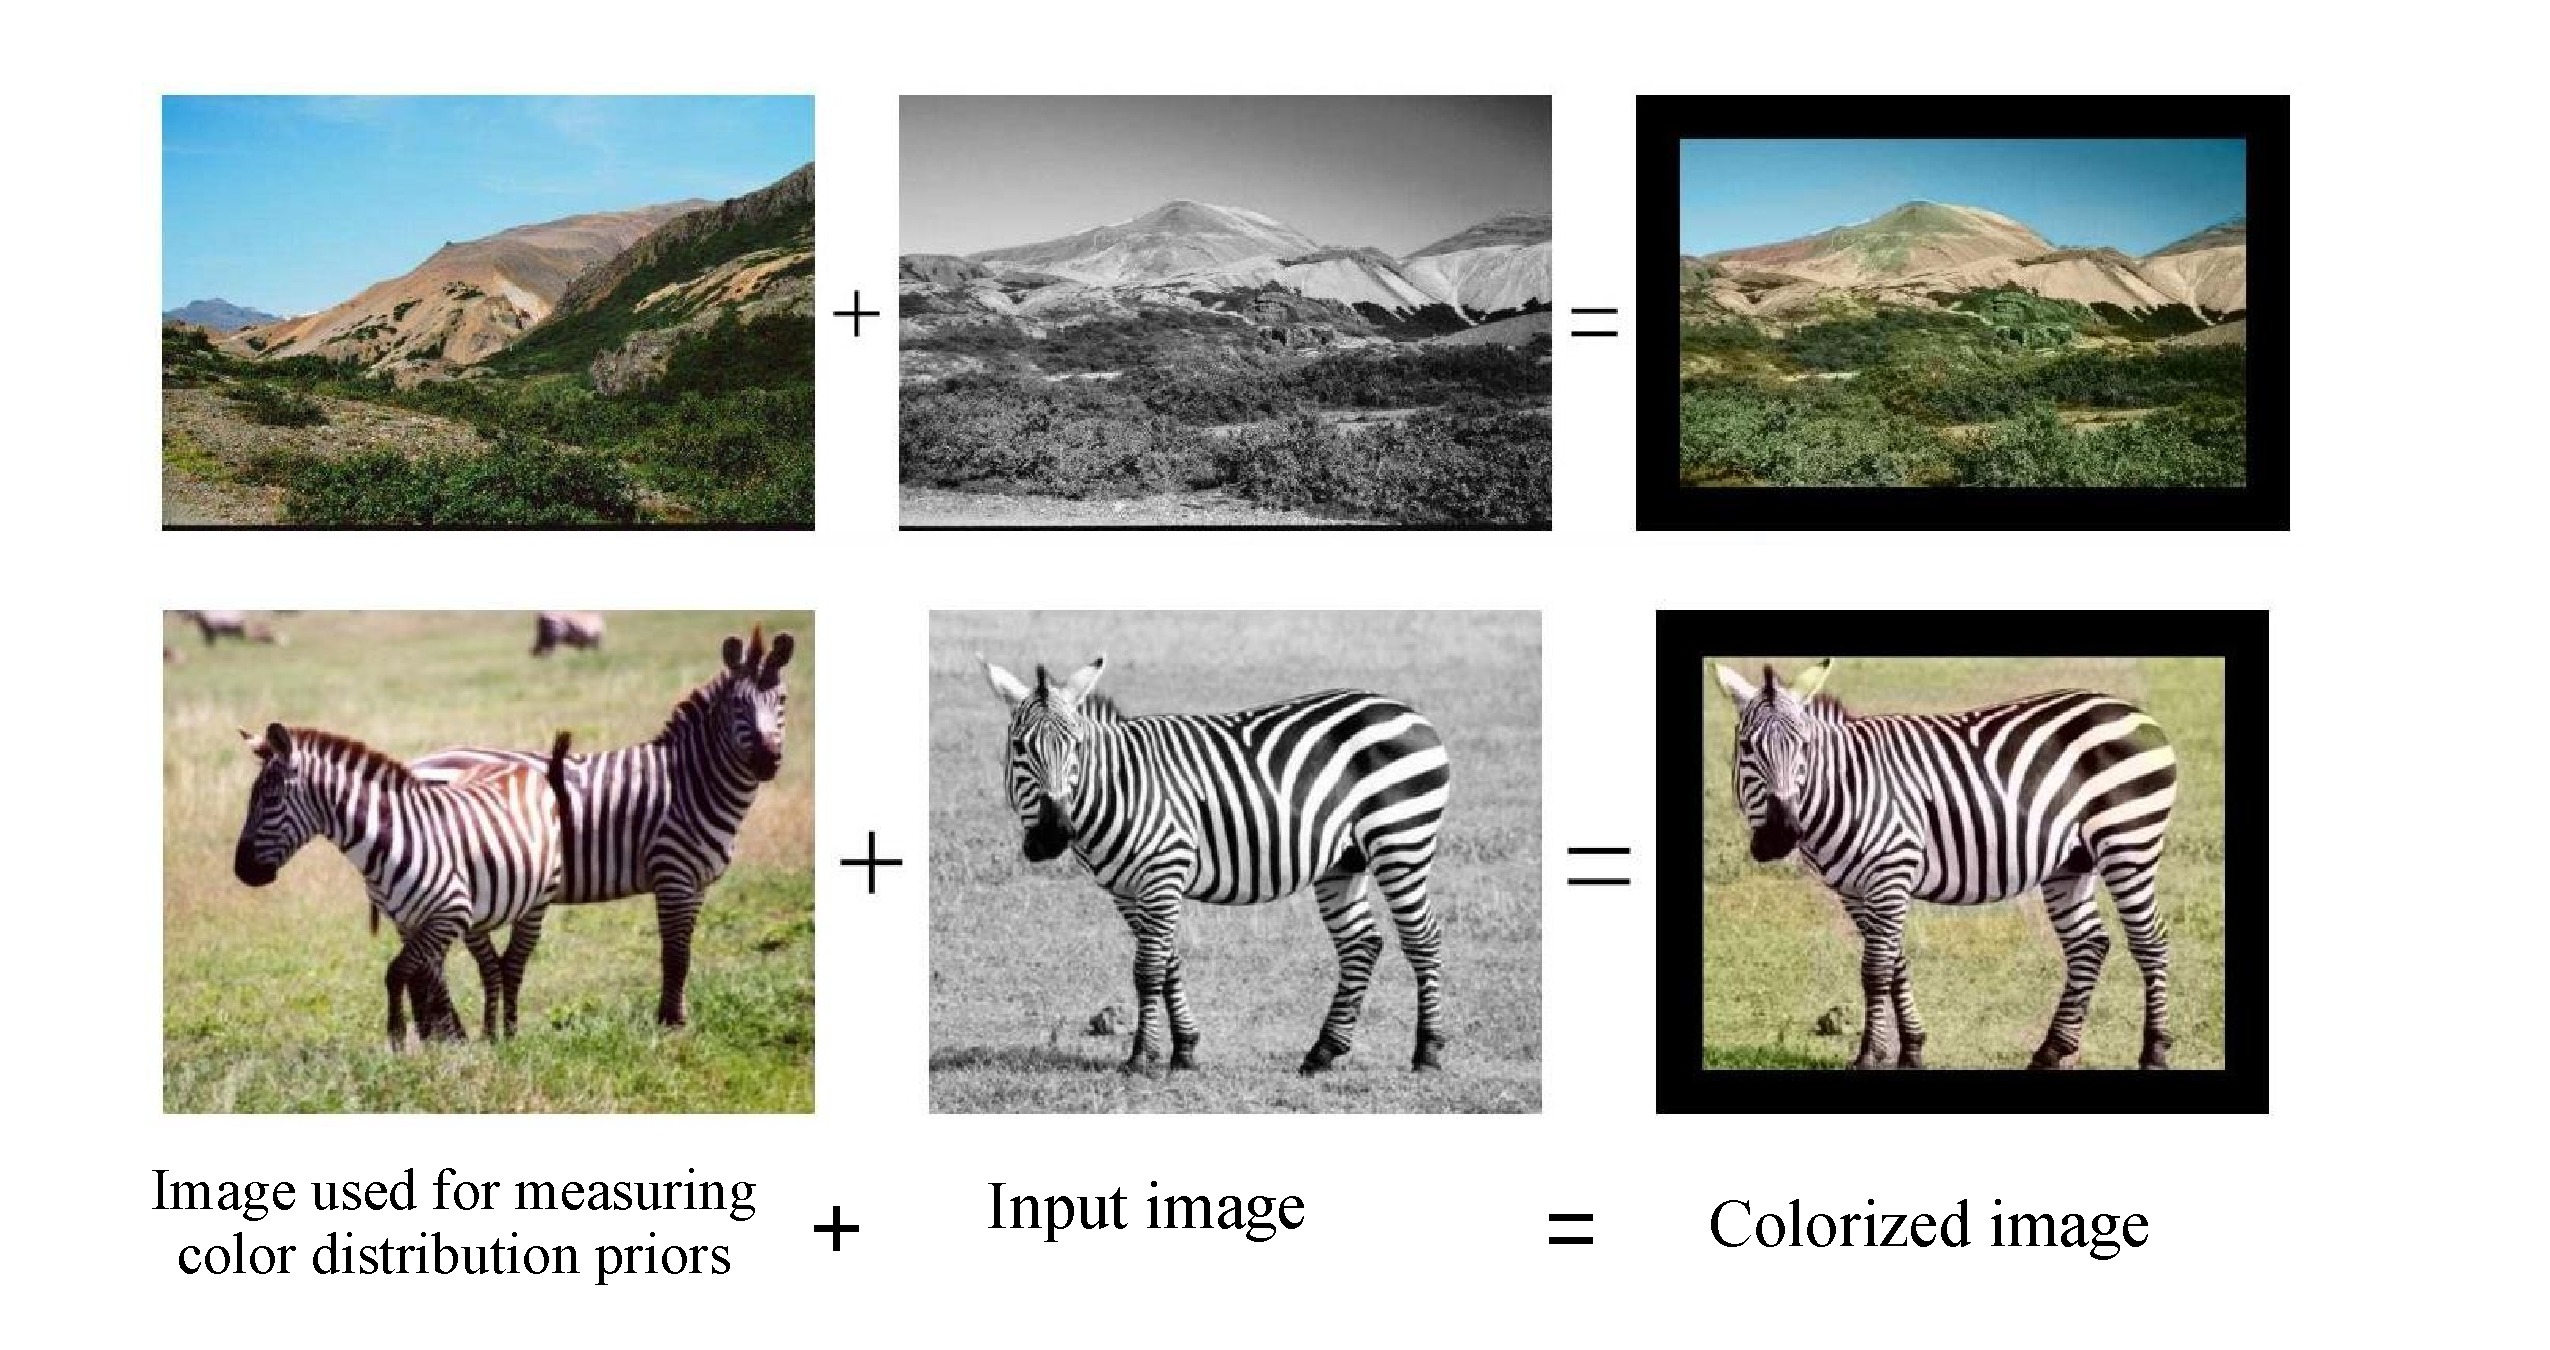
\includegraphics[width=\linewidth]{Figs/52.pdf}
\vspace{-10mm}
\caption{Demonstrations of how colorization is performed in \cite{charpiat2008automatic}. Color distribution prior is estimated from a given image (or a set of training images); then, color projection based on this distribution is performed to predict colors at each pixel}
\label{fig:res2}
\end{figure} 

 

\subsubsection{Pros and Cons:}
This algorithm is fast and robust to texture noises. However, its colorization performance heavily depends on the color distribution prior; consequently, it often produces desaturated coloring if the given reference images are drastically different compared to the test image(s). 

\subsection{\textbf{Colorful Image Colorization (2016)}}
Colorful image colorization \cite{zhang2016colorful} is considered as a major breakthrough on this problem. Published on 2016, it has managed to set a new benchmark for performance. It is an automatic approach that produces realistic colorizations based on a CNN-based model. Previous approaches have either relied on significant user interaction or resulted in desaturated colorizations. To address these issues, it designed a novel \textit{loss function}, which seem to work very well with its underlying CNN-based architecture. 

Furthermore, this paper introduced a notion of evaluating quality of colorization through a \textit{colorization Turing test}, in which it can fool a human judge $32\%$ of the time. However,  one limitation is that it is not end-to-end trainable (the loss function parameters are approximated separately). As a benchmark, I investigated this model and performed thorough experiments over several datasets, which is discussed next.


\section{Adopted Model, Implementation and Results}\label{sec:res}
Unlike other approaches, colorful image colorization \cite{zhang2016colorful} poses the colorization 
problem as a multi-modal classification problem. The paper presents couple of CNN-based models (one is shown in Fig. \ref{fig:col}, another in Fig. \ref{fig:col_main}), with a novel objective function. The objective function is carefully designed to map the image-to-image translation problem to a classification problem. First, it takes advantage of the fact that $A$, $B$ color components of LAB colorspace for natural images are concentrated in a small region, which can be discretized into finite number of bins ($Q$), as illustrated in the top row of Fig \ref{fig:col_main}. 
Given the lightness channel ($L_p$) of a pixel $p$, its $A$, $B$ pair corresponds to a particular bin (out of $313$ bins in total), which is mapped to a 1-hot vector ($Z_p$). 
Consequently, task of the classification model, is to predict which bin each pixel corresponds to. That is, the output is a $313$-mode probability distribution ($ \hat{Z_p}$) for each pixel $p$. The objective function is modelled as a cross entropy loss between $Z$ and $\hat{Z}$, expressed as follows: 

\[ L_{col}(Z, \hat{Z}) = - \sum_p Z_p \sum_{q \in Q} Z_p[q] log(\hat{Z_p}[q])   \] 

This cross-entropy loss can be further augmented with class rebalancing, to encourage rare colors. The detailed model specification, as shown in the bottom-row of Fig. \ref{fig:col_main}, is an 8-layer CNN architecture where each conv layer refers to a block of $2$ or $3$ repeated
conv and ReLU layers \cite{nair2010rectified}, followed by a BatchNorm layer \cite{ioffe2015batch}. The network has no pool layers; 
all changes in resolution are achieved through spatial down-sampling or up-sampling between conv blocks.


\begin{figure}[h]
\centering
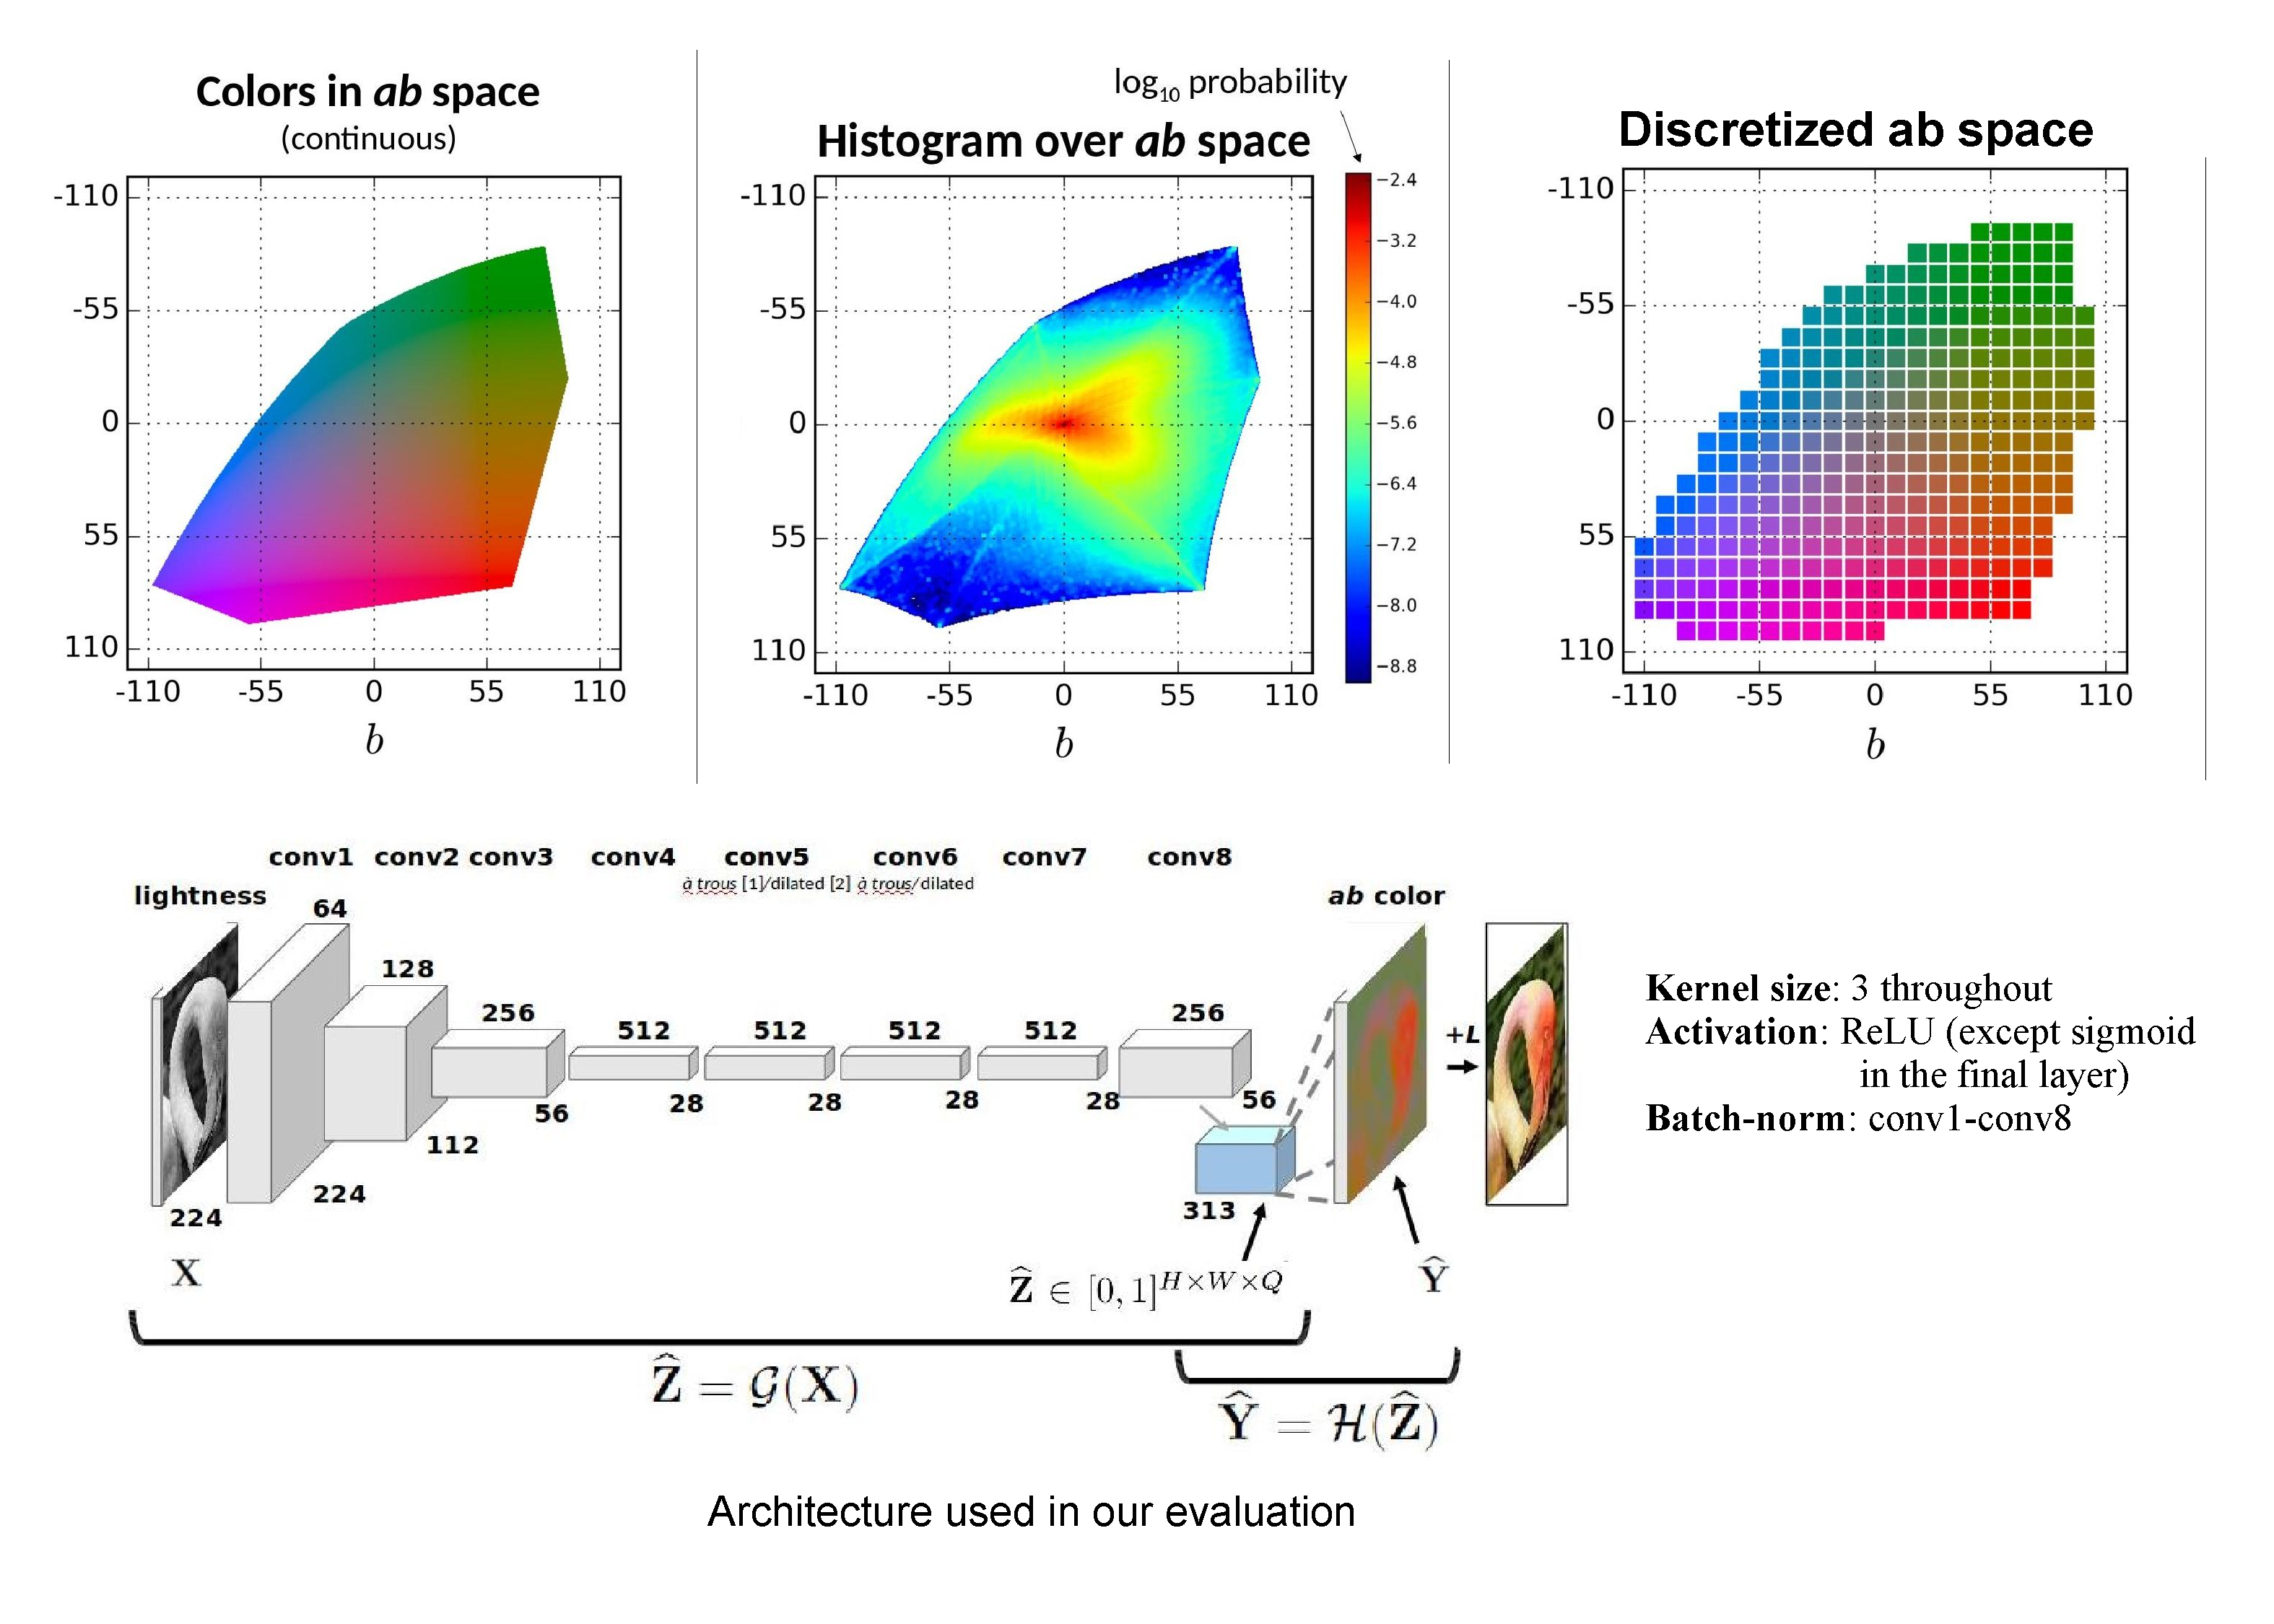
\includegraphics[width=\linewidth]{Figs/9.pdf}
\vspace{-10mm}
\caption{The top row shows how the distribution of $A$, $B$ color components is discretized to finite number of bins; bottom row shows the model architecture adopted in our evaluation. (figures are taken from the paper \cite{zhang2016colorful}; code is available at \cite{ColCol})}
\label{fig:col_main}
\end{figure}  


\subsection{Implementation Details and Results}
While working on designing a generator for our GAN-based model, I investigated this model with different objective functions ($L_1$ loss, $L_2$ loss, least-squared loss, etc.) instead of their cross-entropy based loss function. This is due to the fact that in a GAN-based model, \textit{discriminator} expects an image from the \textit{generator}, 
and tries to discriminate it as real or fake in order to force the generator to get better.  
Therefore, rather than adopting their classification model directly, I implemented their architecture 
using objective functions based on $L_1$, $L_2$, least-squared loss (so that it outputs an image, not classification probabilities). 

Given an input image $I$, the network is fed with its $L$ channel ($I_L$); the output layer of the network is adjusted to predict $\hat{I}_{AB}$. We have found $L_1$ and $L_2$ loss functions perform quite well with this model. These loss functions between true $I_{AB}$ and $\hat{I}_{AB}$ can be expressed as follows:

\[ L_1 (I_{AB}, \hat{I}_{AB}) = \lambda \sum_p | I_{AB}[p] - \hat{I}_{AB}[p] | \]  
\[ L_2 (I_{AB}, \hat{I}_{AB}) = \lambda \sum_p ( I_{AB}[p] - \hat{I}_{AB}[p] )^2 \]  

Here, $\lambda$ is a normalization constant. CelebA datasets \cite{celebA} is used for training primarily, that has $195K$ training examples (a total of  $202K$ images); 
In a separate training, a set of $200K$ images from Places2 dataset \cite{places2} were also used for training\footnote{Larger datasets like ImageNet \cite{deng2009imagenet} and full Places2 challenge dataset were not used for the project due to time constraint; however, we are planning to train our final GAN-based model over these datasets during the summer.}. Training was performed using two $1080$ gpus (in a core-i7 machine having $64$GB RAM); training time for $100K$ iterations with a batch size $32$ was about $2$-$3$ days for each trial. The implementation is done using tensoflow \cite{abadi2016tensorflow} in python.    


\begin{figure}[h]
\centering
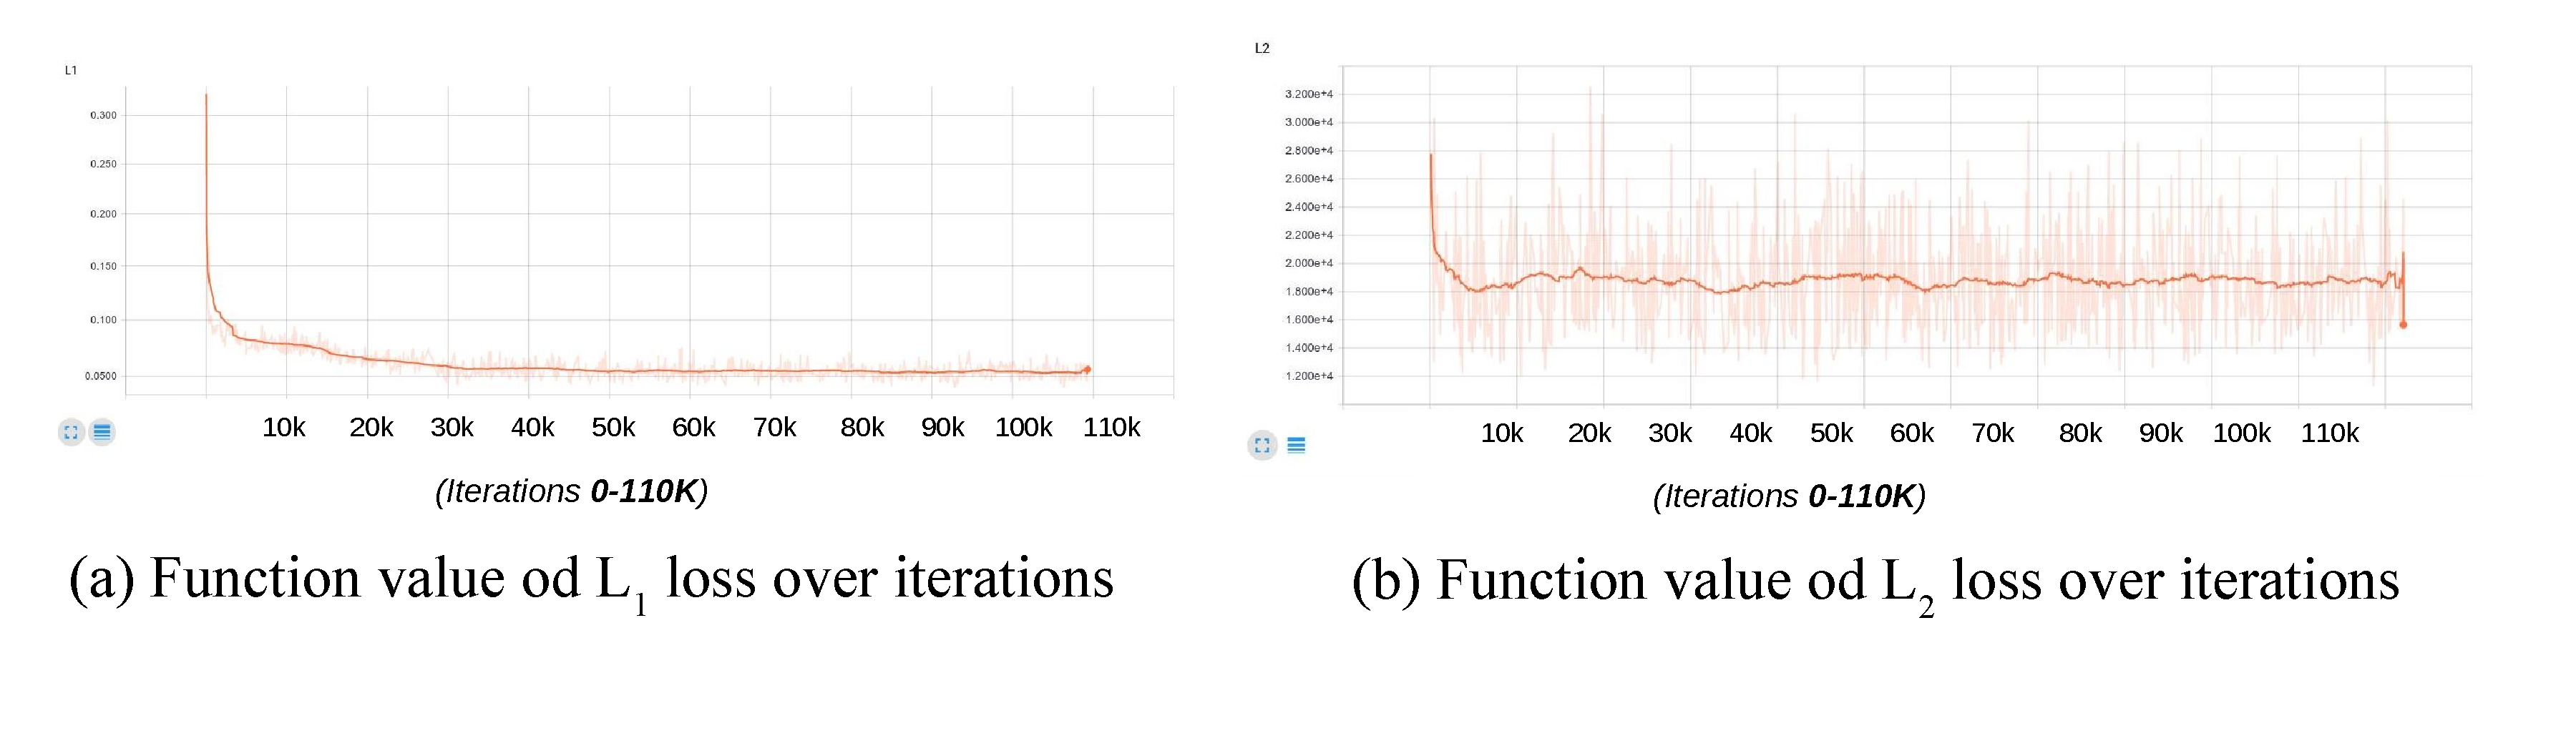
\includegraphics[width=\linewidth]{Figs/8.pdf}
\vspace{-13mm}
\caption{Convergence of different cost functions with the adopted colorization model (as seen on tensor-board)}
\label{fig:loss}
\end{figure}  


\begin{figure}[!h]
\centering
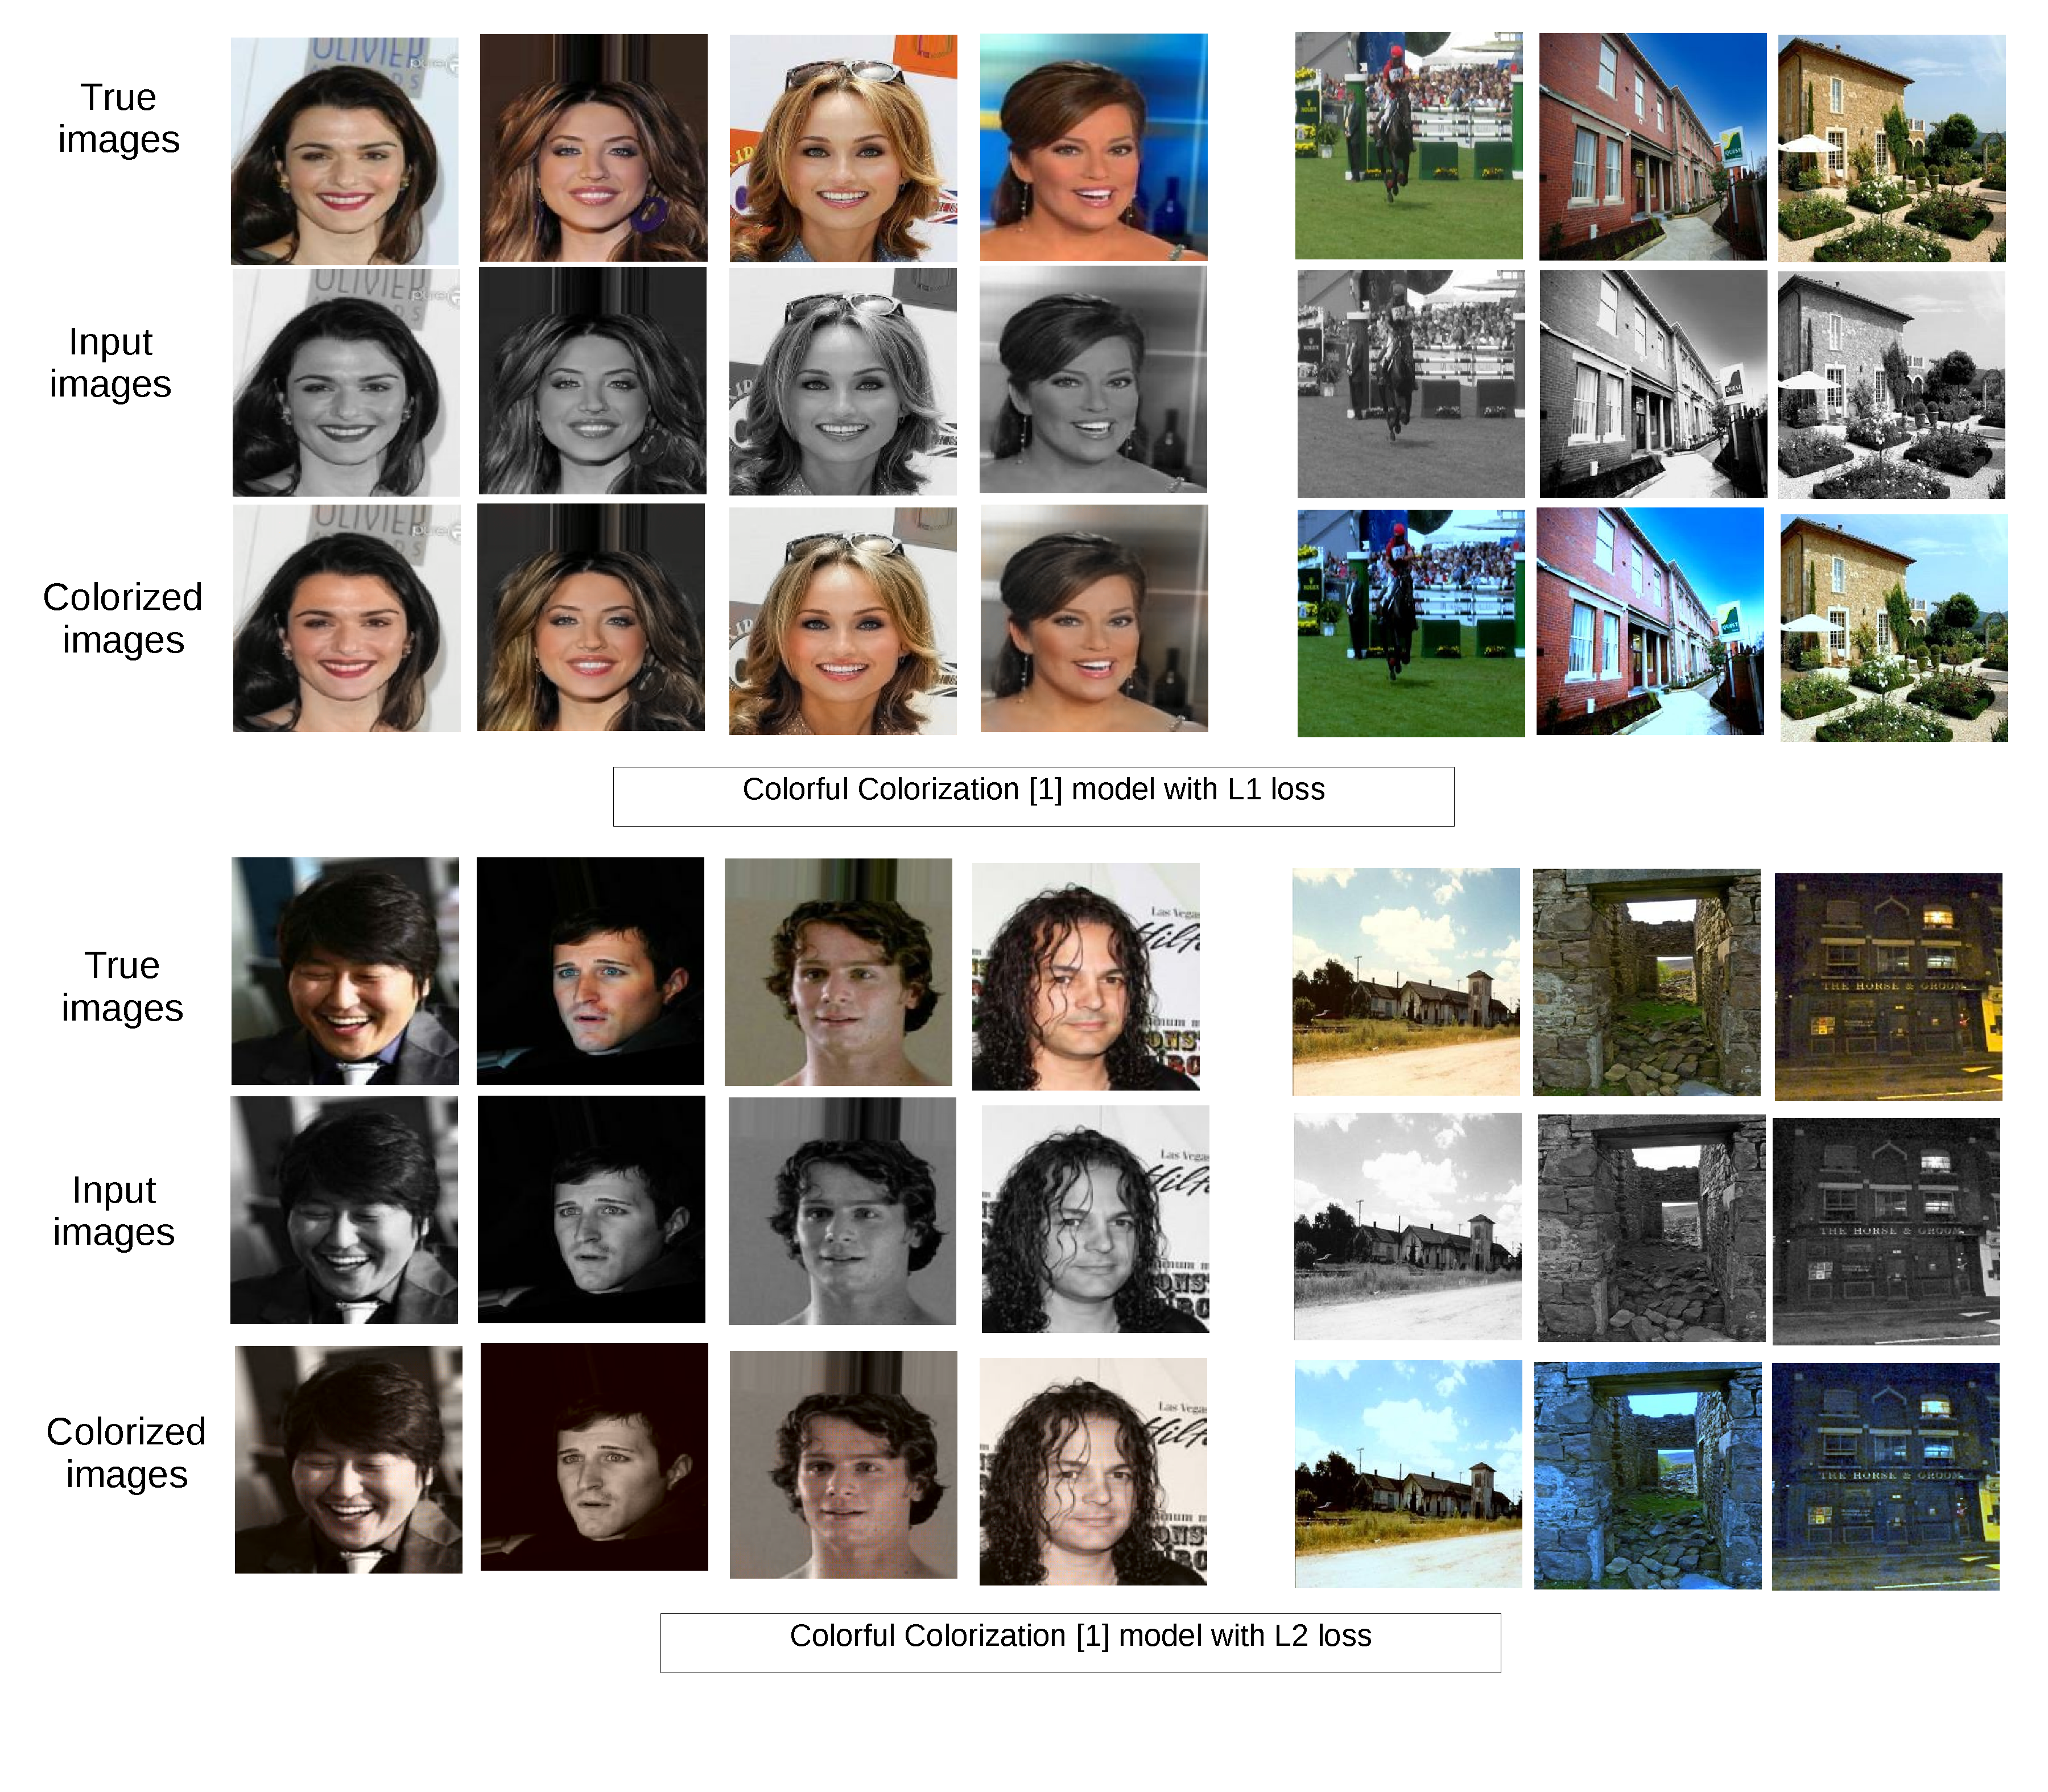
\includegraphics[width=\linewidth]{Figs/4.pdf}
\vspace{-15mm}
\caption{Results for the colorful colorization model \cite{zhang2016colorful} with L1 (top) and L2 loss (top); First $4$ columns show few examples from the test set of CelebA \cite{celebA} dataset, while the rest ($3$) are chosen from test set of Places2 \cite{places2}  dataset }
\label{fig:res_full}
\end{figure}  


We found that this model performs better with $L_1$ loss function compared to $L_2$ loss. Additionally, training is much smoother for $L_1$ loss as well, as evident from Fig \ref{fig:loss}. This might be because of the averaging effect of $2$-norm which causes a blurry colorization (similar phenomena is discussed in \cite{zhang2016colorful}). The results on few test cases are shown in Fig. \ref{fig:res_full}. 

It is to be noted that these results were found while designing it as a generator only, we will discuss results for our GAN-based models in the project report. Currently, the loss function ($L_{col}$) for classification model of the original paper is being tried out, to investigate how it performs over these datasets.    

\subsection{Critics}
As mentioned, the classification model presented in the original paper \cite{zhang2016colorful}  was not directly applicable (as generator) for our GAN-based model. Therefore, we kept it as a image-to-image translation model and tried $L_1$- and $L_2$-loss (instead of cross-entropy based loss) function. Additionally, by doing so, we make this model end-to-end trainable (their proposed model is not end-to-end trainable). Currently, as a generator alone, this model works quite well, specially with $L_1$ loss function. However, further improvement is possible with other GAN-based models, which will be discussed elaborately in our project report.  

\section{Conclusion}
This report discusses three papers that I explored while designing generator for our GAN-based model (project group: YAL). 
These three algorithms, namely colorization using optimization, colorization via multimodal predictions, and colorful image colorization. The later, being the current state-of-the-art and based on deep-learning, was adopted in our evaluation. The problem formulation is provided, implementation details are discussed and results are presented with necessary illustrations. 

\vspace{1mm}
\bibliographystyle{unsrt}
\footnotesize
\bibliography{cvbibs}

\end{document}
